\documentclass[12pt, letterpaper, titlepage]{article}
\usepackage[utf8]{inputenc}
\usepackage{geometry}
\usepackage{color,graphicx,overpic,colortbl} 
\usepackage{fancyhdr}
\usepackage{amsmath,amsthm,amsfonts,amssymb}
\usepackage{mathtools}
\usepackage{hyperref}
\usepackage{multicol}
\usepackage{array}
\usepackage{float}
\usepackage{blindtext}
\usepackage{longtable}
\usepackage{scrextend}
\usepackage[font=small,labelfont=bf]{caption}
\usepackage{calc}
\usepackage{titlesec}
\usepackage{listings}
\usepackage[normalem]{ulem}
\usepackage{tabularx}
\usepackage{mathrsfs}
\usepackage{bookmark}
\usepackage{apple_emoji}
\usepackage{setspace}
\usepackage{ragged2e}
\usepackage{ltablex}
\usepackage{xurl}
\usepackage{tikz}
\usepackage{pgfplots}
\usepackage{xparse}

\mathtoolsset{showonlyrefs}  
\allowdisplaybreaks
\lstset{basicstyle=\ttfamily, keywordstyle=\rmfamily\bfseries}

\definecolor{comment}{RGB}{140, 140, 140}
\definecolor{text}{RGB}{0, 0, 0}
\definecolor{string}{rgb}{0.58,0,0}
\definecolor{variable}{RGB}{244, 63, 78}

\lstdefinestyle{code_style}{
    commentstyle=\color{comment},
    keywordstyle=\color{variable},
    numberstyle=\tiny\color{text},
    stringstyle=\color{string},
    basicstyle=\ttfamily\scriptsize\color{text},
    breakatwhitespace=false,         
    breaklines=true,                 
    captionpos=b,                    
    keepspaces=true,                 
    numbers=left,                    
    numbersep=-10pt,                  
    showspaces=false,                
    showstringspaces=false,
    showtabs=false,                  
    tabsize=4
}

\newcolumntype{q}{>{\hsize=.45\hsize}X}
\newcolumntype{e}{>{\hsize=.35\hsize}X}
\newcolumntype{s}{>{\hsize=.15\hsize}X}

\definecolor{mycolor}{rgb}{0, 0, 0}

\geometry{top=2.54cm, left=2.54cm, right=2.54cm, bottom=2.54cm}
\setlength{\headheight}{20pt}
\setlength{\parskip}{0.5cm}
\setlength{\parindent}{1cm}

\pgfplotsset{width=\textwidth-3cm,compat=newest}
\usepgfplotslibrary{patchplots}
\renewcommand{\thesection}{} % Make sections have no number

\newcommand{\B}{
\includegraphics[height=1.5em, valign=B, raise=-0.2em]{BigB.png}} 
\newcommand{\nx}{$n\times1$}

\title{\textbf{\Huge{
    \begin{center}
        ECE 322 Lab Report \#3
    \end{center}
}}}
\author{
\B enjamin Kong \\
1573684 \\
}

\pagestyle{fancy}
\fancyhf{}
\rhead{\thepage}
\lhead{\textit{ECE 322 Lab Report \#3}}

\begin{document} 
\onehalfspacing

\maketitle
\newpage

\section*{Introduction}
The purpose of this lab was to introduce rudimentary techniques of white-box testing, specifically unit testing. Furthermore, this lab introduced pairwise test case generation tools.

Whereas the tester does not know the inner workings of a program when doing black-box testing, for white-box testing, the tester knows the inner workings of the program being tested. This typically means the tester has access to source code. Using this knowledge, the tester can then come up with test cases to test the program. In this lab, we will focus on control flow testing. Control flow testing includes four fundamental coverage criteria: statement coverage, branch coverage, condition coverage, and path coverage. We will be performing control flow testing on a Python program that performs the bisection method (a simple algorithm to solve equations in the form of $f(x)=0$ given an interval in which the root can be found).

In this lab, we also look at pairwise testing. Instead of producing test cases for every possible combination of inputs, pairwise testing makes testing more efficient by allowing testers to construct a set of test cases that covers all combinations of test data for each pair of variables. In this lab, we will be using a pairwise test case generation tool to build a set of test cases. Specifically, in this lab, we will be using allpairspy, a Python library that calculates approximations to orthogonal arrays which are then used to generate test cases. We will be considering a system with three independent variables $A$, \B, and $C$ that take on three possible values 0, 1, and 2.

\section*{Questions}
\subsection*{Q1}
Unit testing is a white-box testing technique. Unit testing is used to verify individual units of code. Typically, in a codebase, individual functions will be tested. Often, each function will have several unit tests in order to test different end cases and scenarios. When a unit test fails, then the tester knows that the function being tested may have an error somewhere. Unit tests should be done as often as possible. We use unit tests because they are helpful for helping developers make sure their changes do not affect other individual units of code. Furthermore, code is typically better designed when testing is done as part of the development process.

\subsection*{Q2}
Code coverage is a metric for measuring the adequacy and completeness of test cases in a given program and is a useful metric to help developers understand how much of their code is tested. It can be a useful metric in assessing test performance and quality of software. There are four fundamental criteria for code coverage: 
\begin{itemize}
    \item Statement coverage: every statement in the code has to be executed at least once,
    \item Branch coverage: every branch in the code has to be executed at least once,
    \item Condition coverage: all possible combinations of conditions in compound decisions must be exercised, and
    \item Path coverage: all possible logical paths must be exercised.
\end{itemize}

\subsection*{Q3}
Pairwise testing is a black-box test technique. Whereas combinational testing produces test cases with every permutation of each input, pairwise testing is significantly more efficient since it produces test cases that covers all combinations of the test data for each pair of variables. Essentially, a subset of all combinations of inputs is produced. While it is not exhaustive, it is still very effective at finding bugs since most defects are caused by interaction of at most two inputs. Furthermore, it produces significantly less test cases than combinational testing.

\section*{Part 1 | Bisect}
\subsection*{Q1}
The bisection method is a simple algorithm that aims to solve equations of the form $f(x) = 0$ when given an interval $x_1 \leq x \leq x_2$ in which the root $x$ can be found. Our function in the program \lstinline{mybisect.py} solves this via iteration. First, the solver is initialized with the function \lstinline{func} and the function is given the variables \lstinline{x1} and \lstinline{x2} which represent the start and end of the interval in which to search for the root. Then, in each iteration, the function 
\begin{enumerate}
    \item Finds the values of the function at the endpoints \lstinline{f1} and \lstinline{f2},
    \item Checks if the root is not found (errors if no root found),
    \item Calculates the midpoint \lstinline{mid} and the value of the function at the midpoint \lstinline{fmid},
    \item Checks whether to change \lstinline{x1} or \lstinline{x2} to \lstinline{mid} depending on the sign of \lstinline{fmid},
    \item Increments the iteration number \lstinline{iterNum}, and
    \item Breaks the iteration if \lstinline{fmid} is within the tolerance or \lstinline{iterNum} has exceeded the maximum iteration count. Otherwise, return to step 1 and repeat.
\end{enumerate}
Once the iteration has ended, the program then checks if the maximum iteration count has been exceeded, throwing an error if it has. Otherwise, it returns the current value of \lstinline{mid}.

\newpage
\subsection*{Q2}
The control flow graph diagram is presented below.
\begin{figure}[H]
    \centering
    \caption{Control flow graph diagram. Numbers represent the line numbers in \lstinline{mybisect.py}.}
    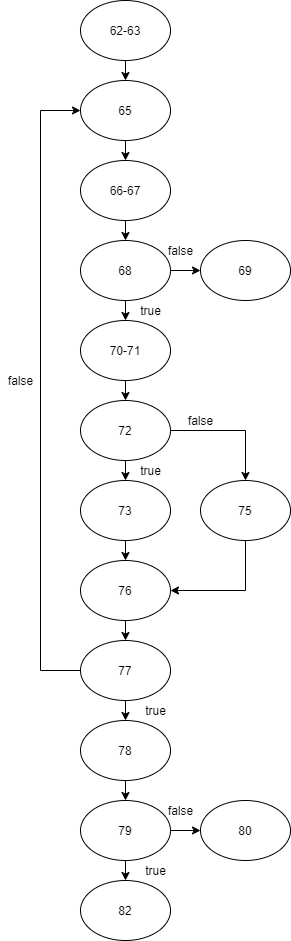
\includegraphics[width=0.35\textwidth]{ControlDiagram.png}
\end{figure}

\subsection*{Q3}
The table is displayed below. The default tolerance is 0.000001 and the default max iterations is 50 unless otherwise stated in the description.

\footnotesize
\begin{centering}
\begin{tabularx}{\textwidth}{|q|X|q|e|e|X|e|}
    \caption{Test cases for \lstinline{bisect.py}} \\ \hline
    \textbf{Test ID} & \textbf{Description} & \textbf{func} & \textbf{x1} & \textbf{x2} & \textbf{Expected} & \textbf{Pass} \\ \hline
    1 & Normal case & $x + 1$ & -10 & 10 & 0 & Y \\ \hline
    2 & Exception when f(x1) \textgreater 0 and f(x2) \textgreater 0 & $x^2+1$ & -10 & 10 & ValueError & Y \\ \hline
    3 & Exception when maximum iterations exceeded & $x$ & -1 & 1e10 & ValueError & Y \\ \hline
    4 & Default constructor (no args) & n/a & -10 & 10 & TypeError & Y \\ \hline
    5 & Custom tolerance (use tol = 10.0) & $x$ & -10 & 10 & 0 & Y \\ \hline
    6 & Custom max iterations (max it = 1000) & $x$ & -1 & 1e10 & 0 & Y \\ \hline
    7 & Custom tolerance \& max iterations (tol = 10.0, max it = 1000) & $x$ & -10 & 10 & 0 & Y \\ \hline
    8 & Getter for tolerance & $x$ & n/a & n/a & tol = 1e-7 & Y \\ \hline
    9 & Setter for tolerance (use tol = 10.0) & $x$ & n/a & n/a & tol = 10.0 & Y \\ \hline
    10 & Getter for max iterations & $x$ & n/a & n/a & max it = 50 & Y \\ \hline
    11 & Setter for max iterations (use max it = 500) & $x$ & n/a & n/a & max it = 5 & Y \\ \hline
\end{tabularx}
\end{centering}
\normalsize

\subsection*{Q4}
The results of running the coverage report in Python are displayed in question 5. Note that the 86\% coverage of \lstinline{mybisect.py} is a result of not testing the \lstinline{main} function as testing \lstinline{main} is practically pointless.
\begin{enumerate}
    \item Statement coverage is relatively easy to obtain, but requires a decent amount of test cases. For example, the getters and setters each had to be called in order to obtain statement coverage for them. Out of the criteria, this was the easiest to achieve.
    \item All branches of the program were tested. It is not too difficult to attain full coverage of all branches, but doing so requires many test cases and some analysis in order to enter all branches. It is a bit of additional work compared to statement coverage.
    \item The tests were able to achieve full statement and branch coverage. Again, the only lines of code that were not tested were from the \lstinline{main} function in \lstinline{mybisect.py}.
    \item No errors were discovered. However, coverage tests do not mean the tests were effective. If more tests were created, errors may be revealed even though we have 100\% coverage.
    \item Path testing would be practically impossible. The number of paths to test is typically $n+1 \leq \text{\#Tests} \leq 2^n$ where $n$ is the number of branches. As we can see, the number of test cases we'd need to complete quickly spirals out of control, making path testing impractical. 
\end{enumerate}

\subsection*{Q5}
The code is provided below.
\begin{lstlisting}[language=Python, style=code_style]
    import unittest
    from mybisect import Polynomial
    from mybisect import MyBisect
    
    class TestMyBisect(unittest.TestCase):
        def test_normal(self):
            # Normal test case
            f = Polynomial(1, 1)  # x + 1
            b = MyBisect(f)
            result = b.run(-10, 10)
            self.assertAlmostEqual(0, f(result), None, 
                                   None, b.tolerance)
    
        def test_both_positive(self):
            # f(x1) > 0 and f(x2) > 0
            f = Polynomial(1, 0, 1)  # x^2 + 1
            b = MyBisect(f)
            self.assertRaises(ValueError, b.run, -10, 10)
    
        def test_exceed_max_iteration(self):
            # Test max iterations exceeded
            # This takes more than 50 iterations
            f = Polynomial(1, 0)  # x
            b = MyBisect(f)
            self.assertRaises(ValueError, b.run, 
                              -1, 100000000000)
    
        def test_default_constructor(self):
            # Test default constructor (no args)
            b = MyBisect()
            self.assertRaises(TypeError, b.run, -10, 10)
    
        def test_tolerance_constructor(self):
            # Test tolerance constructor (tol = 10.0)
            f = Polynomial(1, 0)  # x
            b = MyBisect(10.0, f)
            result = b.run(-10, 10)
            self.assertEqual(0, result)
    
        def test_max_it_constructor(self):
            # Test max iterator constructor (max it = 100)
            # Increasing the max iteration acc should
            # allow us to find the result unlike
            # test_exceed_max_iteration() which reaches
            # the max iteration count.
            # This should take 51 iterations
            f = Polynomial(1, 0)  # x
            b = MyBisect(100, f)
            result = b.run(-1, 100000000000)
            self.assertAlmostEqual(0, f(result), None, 
                                   None, b.tolerance)
    
        def test_tolerance_and_max_it_constructor(self):
            # Test tolerance and max iterator constructor
            # (tol = 10.0, max it = 100)
            f = Polynomial(1, 0)  # x
            b = MyBisect(10.0, 100, f)
            result = b.run(-1, 1)
            self.assertAlmostEqual(0, f(result), None, 
                                   None, b.tolerance)
    
        def test_tolerance_getter(self):
            # Test tolerance getter
            f = Polynomial(1, 0)  # x
            b = MyBisect(f)
            self.assertEqual(0.000001, b.tolerance)
    
        def test_tolerance_setter(self):
            # Test tolerance setter
            f = Polynomial(1, 0)  # x
            b = MyBisect(f)
            b.tolerance = 10.0
            self.assertEqual(10.0, b.tolerance)
    
        def test_max_iterations_getter(self):
            # Test max iterations getter
            f = Polynomial(1, 0)  # x
            b = MyBisect(f)
            self.assertEqual(50, b.maxIterations)
    
        def test_max_iterations_setter(self):
            # Test max iterations setter
            f = Polynomial(1, 0)  # x
            b = MyBisect(f)
            b.maxIterations = 5
            self.assertEqual(5, b.maxIterations)
    
    if __name__ == "__main__":
        unittest.main()
\end{lstlisting}
An image of the coverage report is provided below.
\begin{figure}[H]
    \caption{Coverage report of \lstinline{mybisect.py}. The only relevant value has been marked with a red arrow.}
    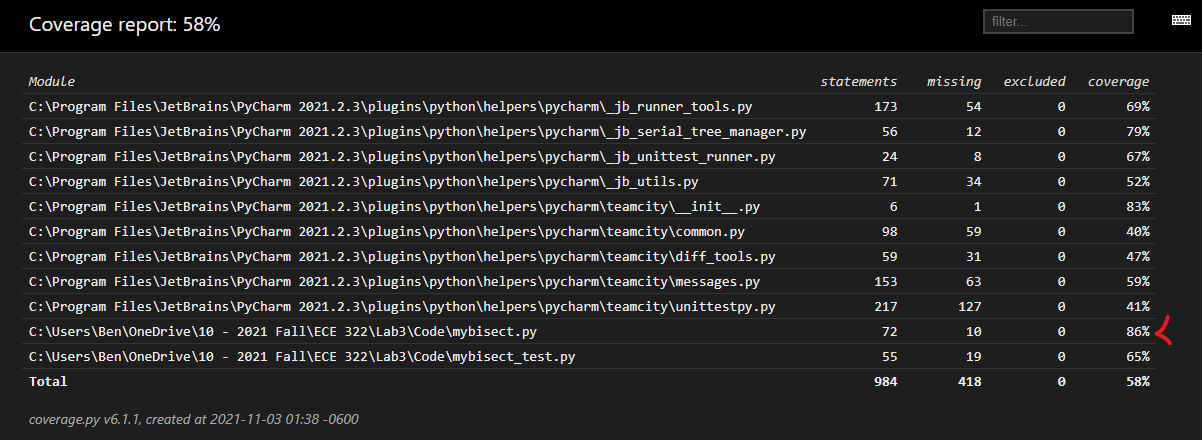
\includegraphics[width=\textwidth]{CodeCoverage1.png}
    \centering
\end{figure}

\section*{Part 2 | Pairwise}
We will be investigating pairwise testing in this section. We will be considering a system with three independent variables $A$, \B, and $C$ that take on three possible values 0, 1, and 2.

\subsection*{Q1}
The closest match was this orthogonal array found at \url{https://www.york.ac.uk/depts/maths/tables/l9.gif}. It had 9 rows and 4 columns, so we simply remove the last column.

\begin{centering}
\begin{tabularx}{\textwidth}{|X|X|X|X|}
    \caption{Test cases from closest orthogonal array.} \\ \hline
    \textbf{Test ID} & \textbf{A} & \B & \textbf{C} \\ \hline
    1 & 0 & 0 & 0 \\ \hline
    2 & 0 & 1 & 1 \\ \hline
    3 & 0 & 2 & 2 \\ \hline
    4 & 1 & 0 & 1 \\ \hline
    5 & 1 & 1 & 2 \\ \hline
    6 & 1 & 2 & 0 \\ \hline
    7 & 2 & 0 & 2 \\ \hline
    8 & 2 & 1 & 0 \\ \hline
    9 & 2 & 2 & 1 \\ \hline
\end{tabularx}
\end{centering}

\subsection*{Q2}
Using the \lstinline{allpairspy} estimation tool, we were able to generate pairwise test cases. This is displayed below. Furthermore, the code is provided in Q4.

\begin{centering}
\begin{tabularx}{\textwidth}{|X|X|X|X|}
    \caption{Test cases from the \lstinline{allpairspy} estimation tool.} \\ \hline
    \textbf{Test ID} & \textbf{A} & \B & \textbf{C} \\ \hline
    1 & 0 & 0 & 0 \\ \hline
    2 & 1 & 1 & 0 \\ \hline
    3 & 2 & 2 & 0 \\ \hline
    4 & 2 & 1 & 1 \\ \hline
    5 & 1 & 0 & 1 \\ \hline
    6 & 0 & 2 & 1 \\ \hline
    7 & 0 & 1 & 2 \\ \hline
    8 & 1 & 2 & 2 \\ \hline
    9 & 2 & 0 & 2 \\ \hline
\end{tabularx}
\end{centering}

\subsection*{Q3}
\begin{enumerate}
    \item Both the custom program and finding an orthogonal array resulted in the same number of test cases. However, finding and modifying the orthogonal array was a little bit more work than generating them using code. 
    \item Both these tools were effective in generating test cases. They were also both equally effective at reducing the number of test cases. Compared to combinational testing, both methods reduced the number of test cases by a factor of 3 (since combinational testing would result in $3\times3\times3 = 27$ test cases).
    \item Pairwise testing is effective at catching errors since many bugs are usually caused by single inputs or the interaction between two inputs. 
    \item Pairwise testing drastically reduces the number of test cases compared with combinational testing. However, it is not as effective as combinational testing as a few edge cases may slip through. For example, a bug may be caused by an interaction between three or more inputs. However, these cases are very rare, and the benefit of drastically reducing the number of test cases makes pairwise testing a good choice in general for testing.
\end{enumerate}

\subsection*{Q4}
The code is provided below.
\begin{lstlisting}[language=Python, style=code_style]
    from allpairspy import AllPairs

    def getallpairspy(parameters):
        print("PAIRWISE:")
        for i, pairs in enumerate(AllPairs(parameters)):
            print("{:2d}: {}".format(i, pairs))

    def main():
        parameters = [
            [0, 1, 2],
            [0, 1, 2],
            [0, 1, 2],
        ]

        getallpairspy(parameters)

    if __name__ == "__main__":
        main()
\end{lstlisting}

\section*{Conclusion}
The purpose of this lab was to introduce rudimentary techniques of white-box testing, specifically unit testing. Furthermore, this lab introduced pairwise test case generation tools.

The first part of this lab focused on coverage testing. There are four fundamental coverage criteria: statement coverage, branch coverage, condition coverage, and path coverage. We also created a control flow graph to analyze the program. By having the source code on hand, we were able to have a detailed analysis of the code. This allowed us to create unit tests that touched all parts of the code. We were able to cover the statement and branch criterion of coverage testing. While coverage testing by itself does not mean the code is error free, it can help show what parts of the code are not tested. When coverage testing is combined with further unit tests and other tests, we have a strong case that the code we have written is error free.

The second part of this lab focused on pairwise testing. Pairwise testing is effective at drastically reducing the number of test cases. We first created test cases by finding an appropriate orthogonal array, then generated test cases using the \lstinline{allpairspy} estimation tool. We found that both these methods were effective at generating pairwise test cases, and that both were equally adept at reducing the number of test cases compared to combinational testing. We also discussed the pros and cons of pairwise testing: pairwise testing drastically reduces the number of test cases, but may let some cases slip through when three or more inputs interact with each other.

\end{document}
